\documentclass{article}
\usepackage[brazil]{babel}
\usepackage[utf8]{inputenc}
\usepackage[pdftex]{graphicx}
\usepackage{caption}
\usepackage{subcaption}
\usepackage{amssymb}
\usepackage{amsmath}
\usepackage[pdftex]{hyperref}
\hypersetup{
    pdfborder = {0 0 0}
}
\usepackage[alf,abnt-etal-cite=2,abnt-etal-list=0,abnt-etal-text=emph]{abntex2cite}

%opening
\author{Ricardo Bustamante de Queiroz}
\title{Tópicos Especiais em Computação Gráfica I\\-- Relatório Final --}

\begin{document}

\maketitle
\tableofcontents

\section{Introdução}

\subsection{Motivação}

Existem diversas soluções para criar animações de personagens articulados. Dependendo da necessidade, técnicas puramente artísticas podem ser utilizadas, onde um modelador define as posições chave, e posições intermediárias são criadas através de interpolações. Esta forma de produzir animações foi inspirada pelo modo que estúdios de animação criavam suas obras desenhando quadro a quadro, e os quadros principais, conhecidos como key frames (Figura \ref{fig:keyframe}), eram desenhados por artistas principais, que guiavam os desenhos dos artístas secundários.

\begin{figure}[ht]
  \centering
  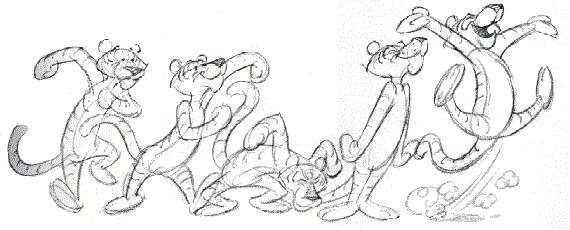
\includegraphics[height=150px]{images/tiger_keys.png}
  \caption{Quadros chave de uma animação tradicional. Imagens intermediárias eram criadas por outros artistas para completar a animação. Na animação por computador, esses quadros intermediários são interpolados a partir dos quadros chave.}
  \label{fig:keyframe}
\end{figure}

Quando há a necessidade de um maior realismo à cena, torna-se difícil contar apenas com o bom senso artístico. Existem duas maneiras mais utilizadas de resolver tal problema.
A primeira consiste em capturar movimentos de um ator real (Figura \ref{fig:mocap}). Toda a naturalidade de seu movimento é traduzida para um avatar virtual, que irá então repetir a mesma movimentação. Comparada com as técnicas tradicionais de animação, a captura de movimentos se assemelha com a rotoscopia. A adversidade desta técnica é quando o mesmo dado de captura é utilizado em uma situação diferente. Caso o modelo representado tenha dimensões diferentes do ator real, ou o ambiente no qual a animação acontece seja modificado, o resultado pode tornar-se estranho ou inconsistente com as regras da física que regem aquele mundo.


\begin{figure}[ht]
  \centering
  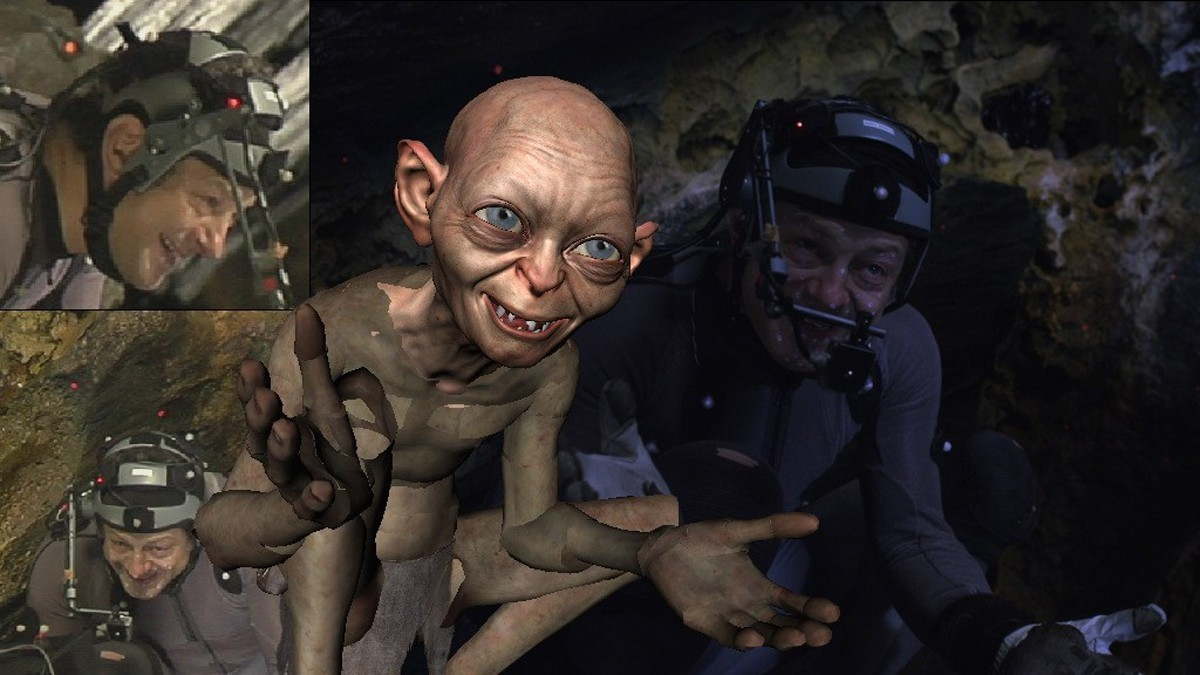
\includegraphics[height=150px]{images/gollum_mocap.jpg}
  \caption{Técnica de captura de movimento. Marcadores acoplados no corpo do ator são registrados por uma câmera ou um sensor, e gravam sua movimentação. Posteriormente, esses dados são utilizados para animar um ator virtual utilizando alguma técnica de computação gráfica.}
  \label{fig:mocap}
\end{figure}

A segunda tenta resolver o problema pensando no realismo. Para isso é necessário ter um modelo físico da cena e do ator virtual. Então, uma simulação física é aplicada, e o produto final é uma animação fisicamente coerente. Apesar do resultado realista, diversos problemas ocorrem. Algumas destas falhas se dão por conta das limitações de uma simulação física no computador. O modelo discretizado será muito mais simples do que sua versão real. As simulações físicas por computador também podem acumular determinados tipos de erros que levam a resultados incoerentes caso os parâmetros não tenham sido devidamente estabelecidos. Outro problema é representar o movimento natural de um ser vivo. A mera simulação não garante essas qualidades, pois muito disso vem da forma como o individuo se desenvolveu, de suas capacidades mentais de controlar sua musculatura e os vícios adquiridos ao longo de sua existência. Tais detalhes, apesar de muitas vezes passarem despercebidos, causam estranhamento se estiverem em falta. \cite{bib:1985:Wilhelms} \cite{bib:1985:Armstrong} Algumas abordagens foram criadas para definir as animações de maneira de mais alto nível. \cite{bib:1994:Panne}

Para tentar conseguir o melhor dos dois mundos, algumas pesquisas tentam juntar o que há de mais importante em cada uma das técnicas citadas \cite{bib:1999:Zordan}. Combinando dados de captura com uma simulação, é possível conseguir animações que capturam a essência do movimento natural sem perder a capacidade de respeitar as restrições do ambiente. \cite{bib:2002:Zordan} Um dos problemas desta forma de tratar o problema, é que o modelo utilizado na simulação física é simplificado. Isso faz com que o personagem, usando apenas o dado de captura como controle, tenha dificuldade de se manter de pé. Algumas técnicas foram desenvolvidas para manter o equilíbrio do avatar diante da simulação, adicionando novos tipos de controle. \cite{bib:2007:Yin} \cite{bib:2012:Geijtenbeek} \cite{bib:2014:Silva}
Nem sempre a animação é previamente definida, seja por um artista ou por uma captura de movimento. Em aplicações interativas, como simulações e jogos, é interessante poder criar uma animação que faça o que se espera, mas sem necessariamente dizer como. O ator virtual deve então, com suas próprias capacidades que foram atribuídas, resolver o problema proposto. O resultado é uma animação que se adapta automaticamente a novas situações. Um exemplo seria um personagem cujo objetivo é atravessar um corredor \cite{bib:2011:Renault}. Porém existem obstáculos neste corredor. E cada obstáculo demanda uma ação diferente para ser transposto. O personagem deve, então, ser capaz de estudar o ambiente e elaborar uma estratégia para percorrer sua trajetória. Outro exemplo é o de um braço mecânico (Figura \ref{fig:roboarm}) que deve capturar uma bola. O desafio é que a bola é arremessada cada vez com uma direção e uma velocidade diferente. O “robô” tem de usar seus sensores para prever a trajetória da bola e interceptá-la. Os dados de captura podem ser utilizados como exemplo para guiar o robô em sua tarefa. Deste modo é possível criar animações complexas definindo apenas em alto nível a solução do problema, sem a necessidade de programar cada caso particular individualmente.

\begin{figure}[ht]
  \centering
  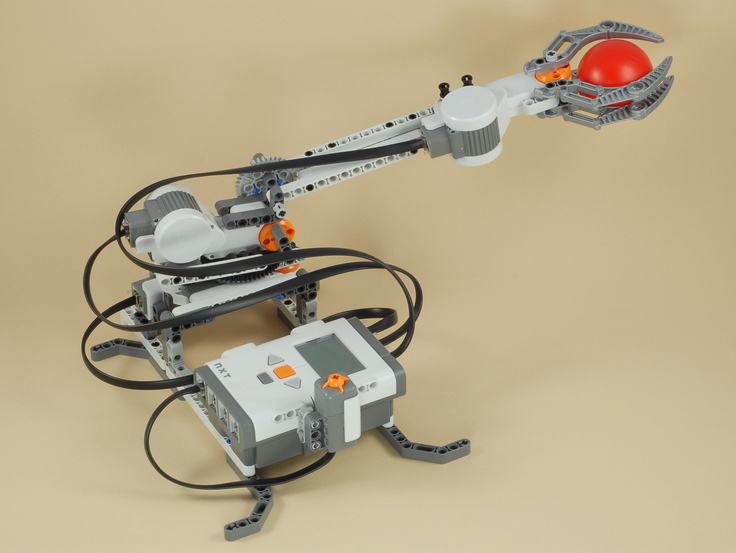
\includegraphics[height=150px]{images/roboarm.jpg}
  \caption{Braço mecânico que pode ser simulado em uma aplicação de realidade virtual. A fase de treinamento do braço na tarefa de captura da bola pode ser realizada em um ambiente de computação gráfica para poupar custo operacional e de tempo.}
  \label{fig:roboarm}
\end{figure}

Para conseguir esses tipos de comportamento, é interessante combinar o uso de algumas técnicas: Inteligência artificial, para que o personagem virtual possa aprender a solucionar o problema, processamento de imagens e outras estratégias para criar o sensoriamento do avatar, e técnicas de animação, para definir os controles que irão manipular o personagem, e até mesmo integrar os comportamentos com animações previamente capturadas.

\subsection{Descrição do problema}

A tarefa a ser realizada é a de descrever o comportamento de uma entidade em relação a um objeto vindo em sua direção. Ela pode então optar por reagir ao estímulo causado pelo objeto, ou ignorá-lo completamente. Caso seja constatado que deve reagir ao objeto, deve então tomar a decisão de aproximação ou afastamento do objeto alvo, dependendo da tarefa a ser realizada. 
Um critério de alcance deve ser definido para que seja possível determinar se o objeto atingiu a entidade ou não, para avaliar o resultado de sua meta. Esse critério vai depender de como a cena foi modelada. O personagem e o objeto podem ser descritos com diversos níveis de complexidade, o que pode dificultar ou até impossibilitar a realização da tarefa com sucesso.
	Exemplo 1 (Figura \ref{fig:hookandhead} A) O personagem deve desviar de um tijolo. Se o ator está parado e um tijolo é arremessado em sua direção, dependendo da velocidade do tijolo e da velocidade máxima que o personagem pode atingir, pode não ser possível que ele desvie. Porém, se for possível, espera-se que o personagem tome uma atitude com este objetivo.
	Exemplo 2 (Figura \ref{fig:hookandhead} B): Um braço mecânico acoplado sobre uma base estática deve capturar uma bola que é jogada em sua direção. O robô possui uma câmera e é capaz de ver a bola. O braço mecânico possui uma área de atuação, que são os lugares onde sua garra é capaz de alcançar. Essa área é limitada pelos ângulos que as juntas do robô são capazes de atingir. Se a bola for jogada de forma que sua trajetória não intercepte a área de atuação do robô, ele não poderá capturá-la. \cite{bib:2011:Hamon}
	
\begin{figure}[ht]
  \centering
  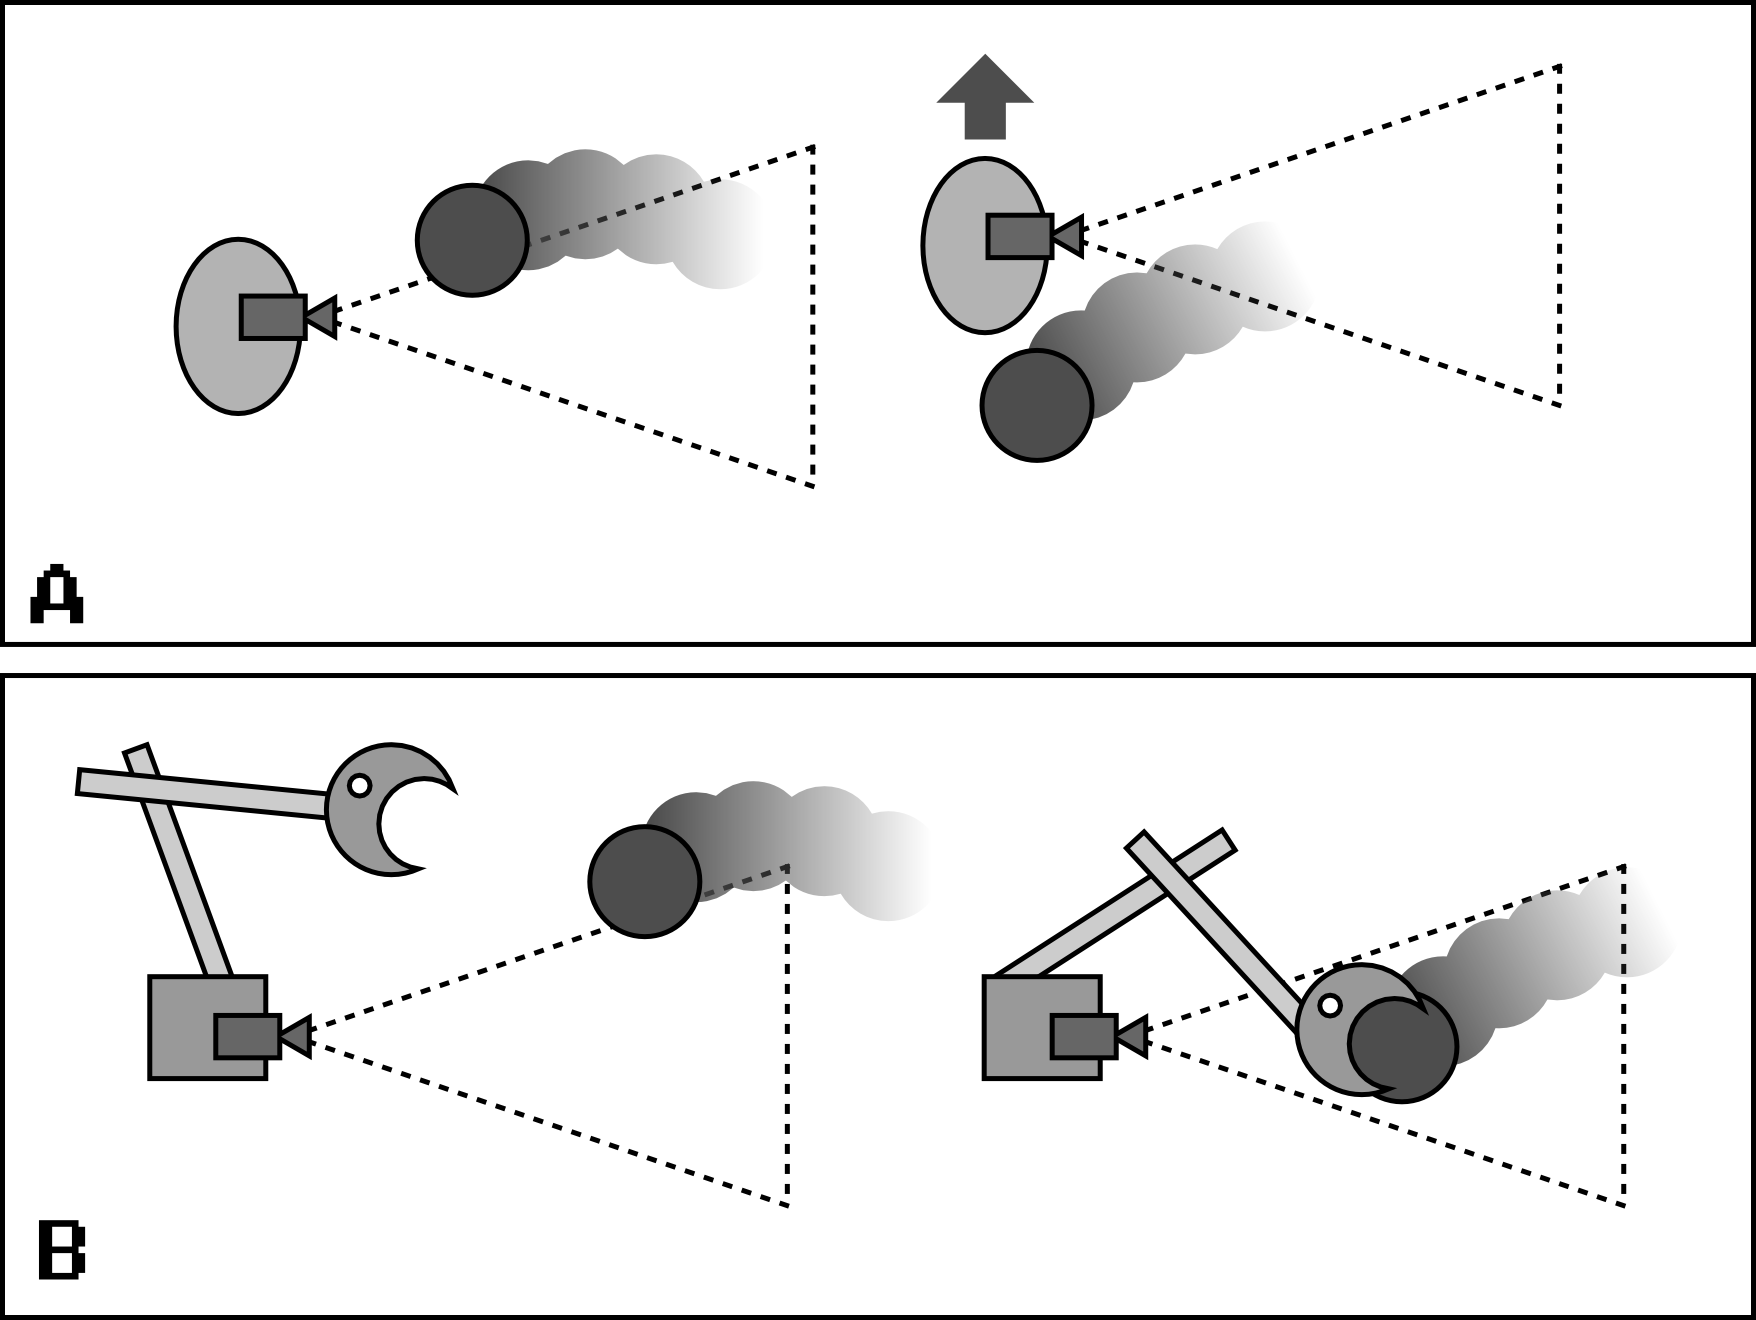
\includegraphics[height=200px]{images/gancho_e_cabeca.png}
  \caption{(A) Uma cabeça, que possui um sensor visual, tenta desviar do objeto jogado em sua direção. Em uma situação onde o personagem tivesse um corpo preso a sua cabeça, a movimentação deslocaria o sistema inteiro. (B) Um braço mecânico tenta agarrar um objeto jogado em sua direção. Nesse exemplo simplificado, a posição da garra e o momento em que ela deve ser acionada não importam. Apenas a sua posição.}
  \label{fig:hookandhead}
\end{figure}
	
	A modelagem dos problemas depende muito de como a solução se desenvolverá. No primeiro caso, se o tijolo atingir qualquer parte do corpo do personagem, seu objetivo foi descumprido. No segundo exemplo, apenas a garra do braço mecânico é capaz de segurar a bola. Alem disso, há diferenças no posicionamento dos sensores, que podem ser móveis ou estáticos, determinar se o personagem deve seguir uma animação pre-definida ou não, entre outros.
O input dos sensores é convertido em uma ação através do uso de controladores. Desta forma, é possível determinar quando, como e para onde o personagem deve se movimentar. O grande problema dessa abordagem é a criação de tais controladores, pois dependendo do nível de controle e o número de sensores que o avatar possa ter, pode se tornar uma tarefa extremamente complexa.
Para solucionar esse problema, existe a ideia de fazer uso de inteligência artificial para programar os controladores. Diversos artigos abordam maneiras diferentes de conseguir isto. A mais comum é fazendo o uso de redes neurais, onde a rede tem como entrada o input dos sensores, e como saída, um sinal para os controladores. Dessa forma é possível treinar o sistema para realizar uma determinada tarefa.
Uma vez que o sistema está treinado e funcionando como deveria, é possível combinar a animação do avatar resultante com outras técnicas de animação. Dependendo de como o sistema for modelado, é possível utilizar um objeto treinado para desviar ou alcançar um obstáculo como efetor final de uma cadeia articulada, e fazendo uso de cinemática inversa, criar uma animação para todo o corpo.

\section{Trabalhos Relacionados}

\subsection{Teaching a robot to grasp}
\citeonline{bib:2011:Hamon} descreve uma técnica para ensinar um braço mecânico (Figura \ref{fig:hamon:fig1}) a capturar uma bola arremessada. O controle do robô é realizado por uma rede neural (Figura \ref{fig:hamon:fig2}), que recebe como entrada um vetor correspondente a velocidade inicial da bola, e fornece como saída a posição em que o gancho deve estar. Como a mesma é sempre jogada da mesma posição, é possível só com isso, prever o local em que o gancho do robô deve estar. Movimentos humanos são capturados e servem como entrada para o algoritmo, que irá utilizar os dados para construir a rede. Além dos dados fornecidos explicitamente, mais dados são gerados interpolando os existentes, produzindo novos casos. Uma vez treinada, a rede foi capaz de demonstrar resultado com uma taxa de captura de aproximadamente 90\%, semelhante a conseguida pelo ser humano. O fato do programa usar a velocidade inicial da bola como sensor é uma simplificação do problema real, onde este dado deveria ser extraido de algum lugar, como uma câmera acoplada no robô.

\begin{figure}[ht]
  \centering
  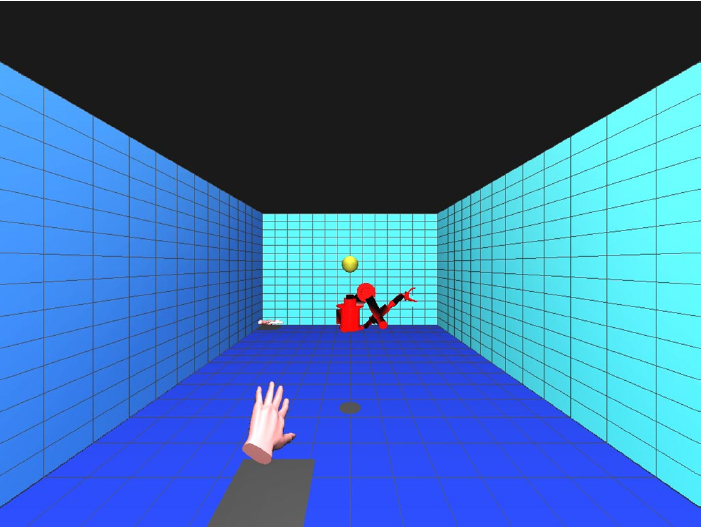
\includegraphics[height=100px]{images/teaching_env.png}
  \caption{Ambiente virtual de \citeonline{bib:2011:Hamon}. A bola arremessada deve ser capturada pelo braço mecânico.}
  \label{fig:hamon:fig1}
\end{figure}

\begin{figure}[ht]
  \centering
  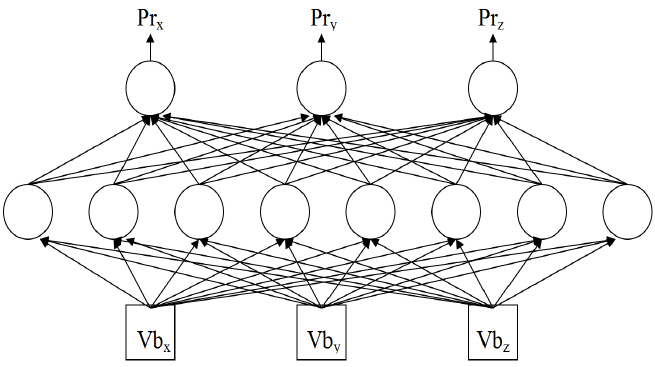
\includegraphics[height=100px]{images/teaching_neural.png}
  \caption{Rede neural usada por \citeonline{bib:2011:Hamon}}
  \label{fig:hamon:fig2}
\end{figure}

\subsection{Trajectory Prediction}
\citeonline{bib:1995:Payeur} descreve como prever a trajetória de um objeto utilizando seu posicionamento. As posições ao longo do tempo são registradas, e utilizadas como entrada para uma rede neural. Essa fornece como saída as coordenadas antecipadas do objeto (Figura \ref{fig:payeur:fig1}). Para o treinamento da rede podem ser utilizadas trajetórias reais de objetos, ou descrições analíticas de uma trajetória. Uma vez que um conjunto de dados é definido, eles são normalizados e restritos a um conjunto limitado para diminuir o espaço de busca. A técnica utilizada para treinar a rede é o algoritmo backpropagation.

\begin{figure}[ht]
  \centering
  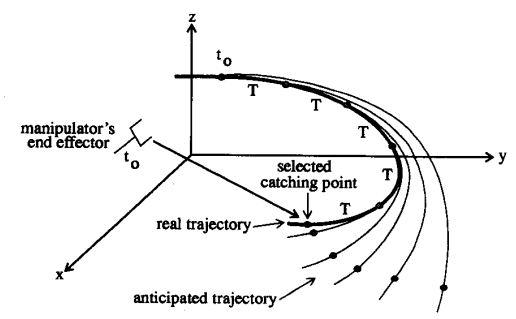
\includegraphics[height=150px]{images/payeur_trajectory.png}
  \caption{Trajetória antecipada do objeto. A cada intervalo de tempo T, é feita uma medida, e o valor antecipado se aproxima do real.}
  \label{fig:payeur:fig1}
\end{figure}

\subsection{Emergent Behavior}
\citeonline{bib:2013:Nogueira} trata de um problema menos definido. A ideia é provar que o comportamento é capaz de se manifestar naturalmente a partir de um agente (Figura \ref{fig:nogueira:fig1}) e do mundo onde vive. Uma vez definido o agente, e as regras de interação com o meio, uma simulação é realizada para desenvolver o comportamento. Os seres capazes de sobreviver ao meio passam suas características a diante, o que representa, em gerações futuras, a emergência de comportamentos que parecem naturais e inteligentes. Um dos fatores mais interessantes deste trabalho é que os personagens, ou agentes, possuem sensores visuais simplificados, que apenas indicam a distância para um determinado obstáculo.

\begin{figure}[ht]
  \centering
  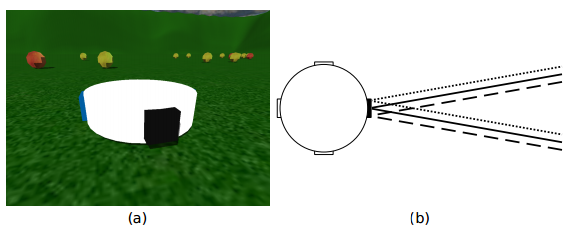
\includegraphics[height=100px]{images/nogueira_robot.png}
  \caption{O robô de \citeonline{bib:2013:Nogueira}. (a) A caixa preta representa tanto o sensor visual, como a boca do robo. (b) Ilustra os três sensores visuais, capazes de informar apenas a distância normalizada para um determinado obstáculo. A distância máxima de sensoriamento corresponde a seis vezes o diâmetro do robô. }
  \label{fig:nogueira:fig1}
\end{figure}

\subsection{Vision-based behavioral animation}
\citeonline{bib:2011:Renault} elaborou uma técnica para guiar o comportamento de um personagem virtual baseado em sua visão. Um conjunto de ações é previamente definido, associando uma determinada situação a uma animação. O ator possui um sistema de navegação, que baseado em seu input visual, é capaz de definir uma ação a ser tomada. Um exemplo é a forma de caminhar, que pode mudar dependendo de outros atores que estejam em seu campo de visão. O personagem é capaz, também, de desviar de obstáculos e encontrar o seu destino final baseado no que consegue enxergar. O sistema de navegação nada mais é do que um mapa que relaciona determinadas características na imagem capturada com a ação a ser tomada. Porém a visão utilizada no artigo é simplificada, pois muitas etapas de reconhecimento de padrões e detecção de distância são puladas, utilizando a vantagem do ambiente estar modelado no mesmo sistema em que o agente se encontra. Cada estado de comportamento em que o personagem pode estar é programado individualmente, tirando parte da autonomia do sistema e tornando o processo um tanto quanto trabalhoso. Entretanto a animação resultante é mais próxima do esperado.

\subsection{Ball tracking}
\citeonline{bib:2009:Birbach} compõe um modelo matemático e estatístico para solucionar o problema de rastreio de uma ou mais bolas utilizando uma câmera. Com tal processamento, é possível extrair de imagens capturadas por um robô ou agente virtual informações melhores para utilizar como entrada para uma rede neural. O artigo cita que o sistema precisa ser calibrado com o tamanho da bola, pois sua distância é estimada a partir do raio que a mesma aparece na imagem capturada. A bola é encontrada na imagem a partir de um algoritmo relativamente simples, que verifica se todos os pontos semelhantes estão igualmente distantes de um determinado ponto. Deste modo é possível calcular a posição do centro da esfera.

\subsection{Autonomous robot guidance}
\citeonline{bib:1991:Pomerleau} descreve como utilizar imagens capturadas por uma câmera para guiar um carro robô. Uma câmera acoplada no veículo registra imagens da estrada, que são alimentadas em uma rede neural treinada para definir alguns parâmetros de controle do carro, como ângulo do volante e aceleração. Redes neurais especializadas (Figura \ref{fig:pormeleau:fig1}) são separadas em módulos diferentes para facilitar o processo de treinamento. As redes resultantes deste processo são combinadas para formar o sistema de controle.

\begin{figure}[ht]
  \centering
  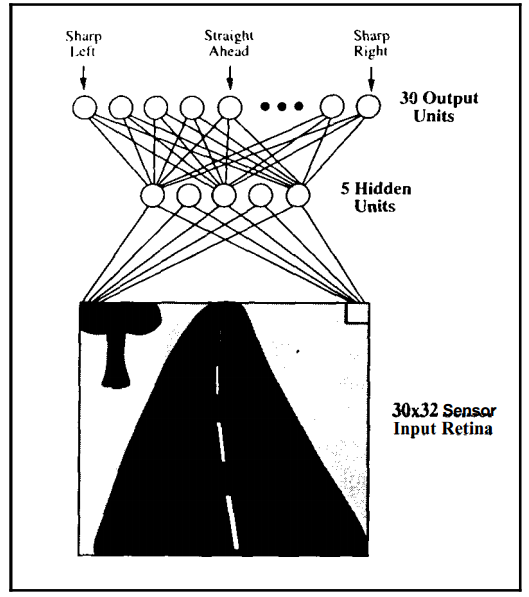
\includegraphics[height=150px]{images/pormeleau_arch.png}
  \caption{Arquitetura de um único módulo de controle. Uma imagem da estrada é dada como entrada, e isso irá definir o ângulo que o veículo deve estabelecer para seu volante.}
  \label{fig:pormeleau:fig1}
\end{figure}

\subsection{Obstacle avoidance}
\citeonline{bib:1997:Nourbakhsh} consegue extrair informações de profundidade de um input visual baseado no foco. Câmeras fotográficas modernas adaptam seu foco de acordo com a entrada de luz. Ele descreve o auto-foco das câmeras como uma solução robusta e eficiente para um sensor ativo de profundidade. Ele descreve então como aperfeiçoar as limitações desse sistema, que permitem apenas um nível de foco por imagem, para prever a profundidade de objetos na cena inteira. A aplicação direta é a criação de um robô equipado com câmeras capaz de desviar de obstáculos.

\section{Problemas possíveis}

Diversos problemas de animação e realidade virtual podem ser solucionados utilizando uma combinação das técnicas citadas.

Fazer um personagem virtual desviar de obstáculos vindo em sua direção é uma aplicação direta. A forma como ele irá desviar pode depender de diversos fatores, como a velocidade no qual o projétil se aproxima.

Outra possibilidade é o problema inverso. Ao inves de desviar de um projétil, o objetivo é antingi-lo. A solução é a mesma do problema anterior, apenas definindo um comportamento diferente para o ator.

Uma adição que pode ser feita é utilizar o ator como um efetor final de um corpo articulado, possibilitando, por exemplo, modificar a animação de um avatar articulado que está seguindo a animação de uma captura de movimento.

Utilizando a ideia de ações pre-definidas para determinadas situações, talvez seja possível combinar diferentes animações capturadas para compor uma animação resultante que seja realista.

\begin{figure}[ht]
  \centering
  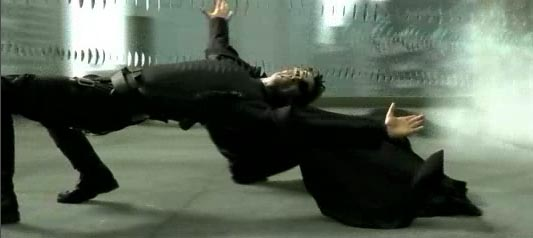
\includegraphics[height=100px]{images/the-matrix-bullet.jpg}
  \caption{Cena do filme The Matrix(1999). Possível cena a ser reproduzida pelo sistema imaginado. Um personagem virtual parado poderia tomar ações drásticas para desviar de um projétil disparado em sua direção. Em uma situação normal, o personagem iria perder o equilíbrio e tombar. O realismo da animação pode ser deixado de lado para criar cenas interessantes dignas da ficção científica.}
  \label{fig:matrix}
\end{figure}

\section{Considerações do relatório}

Tenho muito a melhorar na escrita de relatórios. Talvez não tenha sido formal o suficiente para tratar determinados assuntos, o que pode prejudicar a compreensão do leitor.

A formatação do relatório deixou a desejar. É preciso averiguar melhor o tamanho das imagens, e quando de fato elas são necessárias.

A mudança de tema na metade do caminho fez com que muitos assuntos fossem tratados em um mesmo relatório. Tentei interconectar os assuntos na parte de trabalhos relacionados.

É preciso encontrar um melhor corretor ortográfico. O software que estou utilizando não está devidamente configurado para o idioma Português.

Talvez o relatório tenha ficado muito curto por conta das limitações de tempo, das outras disciplinas e outras atribuições.

O problema final, da captura ou esquiva de um objeto parecem estar mais relacionados com problemas de robótica e inteligência artificial do que problemas de animação ou realidade virtual. Talvez seja interessante trazer a motivação de outras áreas para a computação gráfica.

\bibliography{bib}

\end{document}